\documentclass[25pt, a1paper, landscape, innermargin=-2in]{tikzposter}

% required packages
\usepackage{amsmath}
\usepackage{amsfonts}
\usepackage{amsthm}
\usepackage{graphicx}
\usepackage{natbib}
\usepackage{url}
\usepackage{booktabs}
\usepackage{geometry}

% set the appropriate paper size
\geometry{papersize={42in,40in}}

% compact bibliography
\renewcommand{\bibsection}{}
\setlength{\bibsep}{0pt plus 0.3ex}

%% Available themes: see also
%% https://bitbucket.org/surmann/tikzposter/downloads/themes.pdf

\definecolorpalette{sampleColorPalette} {
  \definecolor{colorOne}{named}{green}
  \definecolor{colorTwo}{named}{black}
  \definecolor{colorThree}{named}{cyan}
}
\usetheme{Default}
%% \usecolorstyle{Denmark}
\colorlet{backgroundcolor}{white}
\colorlet{framecolor}{gray}
\colorlet{blocktitlebgcolor}{gray}

% title information
\title{Guidance on Individualized Treatment Rule Estimation in High Dimensions}
\author{Philippe Boileau$^1$, Ning Leng$^2$, Sandrine Dudoit$^3$}
\institute{$^1$McGill University; $^2$Genentech Inc; $^3$University of California, Berkeley}

% dictate default block options
\newcommand{\myblock}[2]{\block[titleinnersep=2mm, linewidth=0.5mm]{#1}{#2}}
\newcommand{\mysmallblock}[2]{\block[titleinnersep=1mm, linewidth=1mm, bodyinnersep=5mm, roundedcorners=12, ]{{\small #1}}{{\tiny#2\par}}}

% turn off
\tikzposterlatexaffectionproofoff
\begin{document}
\maketitle[width=34in]
%% \node[anchor=west] at (TP@title.west) {
\includegraphics[width=6cm]{logos/mcgill_sig_red}};
%% \node[anchor=east] at (TP@title.east) {
\includegraphics[width=6cm]{logos/cal}};


\begin{columns}

  \column{0.333}

  \myblock{Motivation}{
    \begin{itemize}
      \itemsep2pt
        \item First Item
    \end{itemize}
  }

  \column{0.334}

  \myblock{Estimators}{

    The following conditional average treatment effect (CATE) estimators were
    used to construct the ITR estimators:

    \begin{tikzfigure}
      \centering
        \begin{tabular}{
            |p{3in} || p{8in}|
          }
          \hline
          CATE Estimator
          & Details \\
          \hline\hline
          Plug-In LASSO
          & A plug-in estimator using the LASSO. \\
          \hline
          Plug-In XGBoost
          & A plug-in estimator using XGBoost. \\
          \hline
          Modified Covariates LASSO
          & A modified covariates estimator using the LASSO. The propensity
          score is estimated using the logistic LASSO. \\
          \hline
          Modified Covariates XGBoost
          & A modified covariates estimator using XGBoost. The propensity
          score is estimated using the logistic LASSO. \\
          \hline
          Augmented Modified Covariates LASSO
          & An augmented modified covariates estimator using the LASSO. The propensity
          score is estimated using the logistic LASSO. \\
          \hline
          Augmented Modified Covariates XGBoost
          & An augmented modified covariates estimator using XGBoost. The propensity
          score is estimated using the logistic LASSO. \\
          \hline
          AIPW-based LASSO
          & An AIPW-based estimator using Super Learners to estimate the
          expected conditional outcome and the propensity score. Differences
          in predicted pseudo-outcomes are modelled using the LASSO. \\
          \hline
          AIPW-based Super Learner
          & An AIPW-based estimator using Super Learners to estimate the
          expected conditional outcome and the propensity score. Differences
          in predicted pseudo-outcomes are modelled using a Super Learner. \\
          \hline
          Causal Random Forests
          & A causal random forest estimator using cross-validation for
          hyperparameter selection. \\
          \hline
      \end{tabular}
    \end{tikzfigure}
  }

  \myblock{Simulated Data-Generating Processes}{

    ITR estimators were benchmarked on 16 data-generating processes with
    continuous outcomes and binary treatment assignments reflecting a diversity
    of randomized and observational studies.

    Realizations of random vector $O = (W, A, Y)$ were generated for each
    data-generating process, where $W$ is a random vector of $500$ pre-treatment
    covariates (and possible confounders), $A$ is a binary treatment indicator,
    and $Y$ is the observed continuous outcome. Elements of $O$ are generated as
    follows:
    \begin{align*}
      W & \sim N(0, \Sigma) \\
      A|W & \sim \text{Bernoulli}(\pi(W)) \\
      Y|W, A & \sim N(\mu(W, A), 1) \;.
    \end{align*}
    Here, $\Sigma$ is some $500 \times 500$ covariance matrix, and $\pi(W) =
    \mathbb{P}[A=1|W]$ and $\mu(W,A) \mathbb{E}[Y|W, A]$ are generic propensity
    score and conditional expected outcome functions, respectively. Sixteen
    data-generating processes are defined using combinations of the following
    factors:
    \begin{equation*}
      \begin{split}
        \Sigma_{1} & = I_{500 \times 500} \\
        \Sigma_{2} & = \text{Block diagonal} \\
      \end{split}
    \end{equation*}
    \begin{equation*}
      \times
    \end{equation*}
    \begin{equation*}
      \begin{split}
        \pi_{1}(W) & = \frac{1}{2} \\
        \pi_{2}(W) & = \text{logit}^{-1}\left(\frac{W_{1} + W_{2} + W_{3} + W_{4}}{5}\right) \\
      \end{split}
    \end{equation*}
    \begin{equation*}
      \times
    \end{equation*}
    \begin{equation*}
      \begin{split}
        \mu_{1}(A, W) & = A + \gamma^{\top}W + (\delta^{(10)})^{\top}WA \\
        \mu_{2}(A, W) & = A + \gamma^{\top}W + (\delta^{(50)})^{\top}WA \\
        \mu_{3}(A, W) & = \gamma^{\top}W + 2\;\text{arctan}\left\{(\delta^{(10)})^{\top}WA\right\} \\
        \mu_{4}(A, W) & = \gamma^{\top}W + 2\;\text{arctan}\left\{(\delta^{(50)})^{\top}WA\right\} \\
      \end{split}
    \end{equation*}

  }

  \column{0.333}

  \myblock{Results Snapshot}{
    \begin{tikzfigure}
      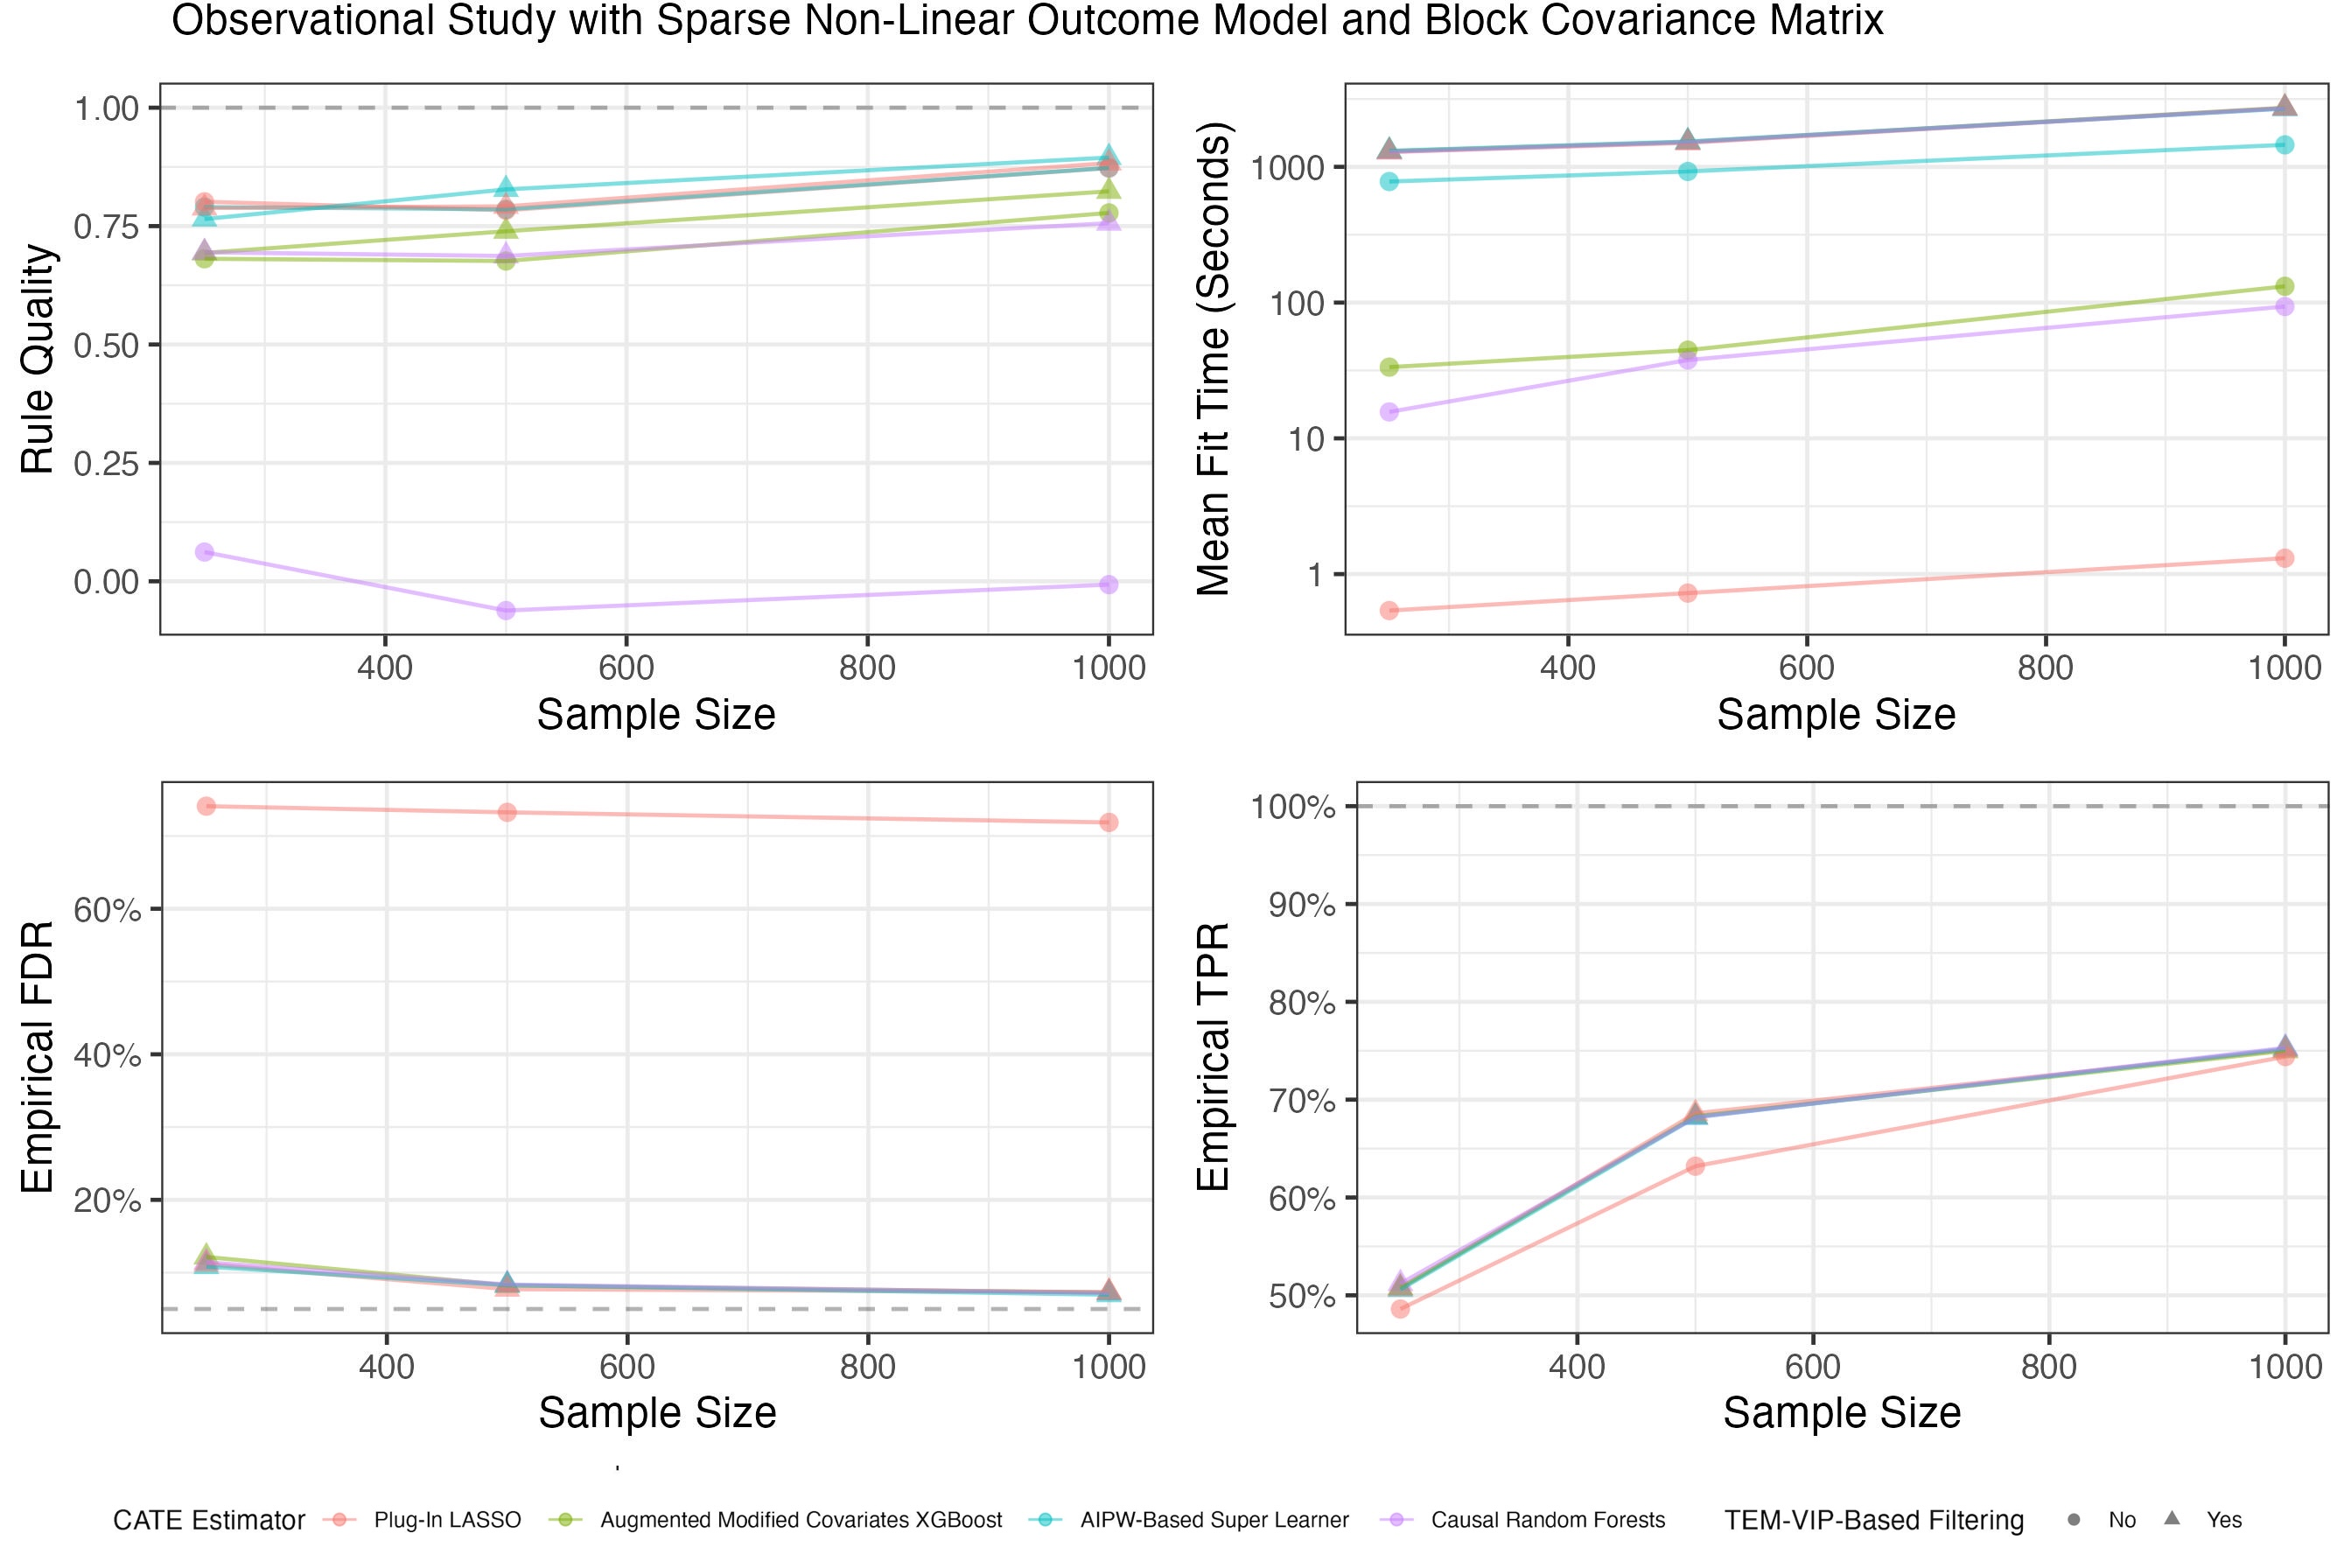
\includegraphics[width=0.29\textwidth]{figs/summary-plot.jpeg}
    \end{tikzfigure}
  }

  \myblock{Practical Guidance}{

    \textbf{No estimator uniformly dominates others across all operating
      characteristics; tradeoffs must be made.} Since rule quality is generally
    of primary concern, practitioners must choose between accurate
    interpretability and computationally efficiency. We provide the following
    guidance on this tradeoff when selecting an ITR estimator for
    high-dimensional data:

    \begin{itemize} \itemsep2pt

    \item \textbf{High-quality rules that are accurately interpretable:} The
      filtered LASSO-based plug-in and AIPW-based estimators generally produce
      high-quality ITR estimates while accurately recovering TEMs. These
      estimators are computationally intensive, however. The computational
      burden might be lestned by parallelizing the estimation procedure.

    \item \textbf{High-quality rules that require few computational resources:}
      The LASSO-based plug-in estimator produces among the most high-quality
      rules in our simulation studies, providing empirical evidence that it is
      robust to model misspecification while being exceptionally computationally
      efficient. This estimator's built-in feature selection capabilities should
      not be used for TEM discovery, however.

    \end{itemize}
  }

  \mysmallblock{References}{
    \vspace{-3em}
    %% \bibliographystyle{unsrtnat}
    %% \bibliography{refs}
    \vspace{-1em}
  }

\end{columns}

\end{document}
